
The sensor cross-sensitivity $\chi$ can be estimated using the FTIR (Fourier
transform infrared) sensor data ($x_1$) along with the actual sensor measrement
data ($y_1$) and the ammonia concentration measurement ($x_2$). We have,
\begin{align*}
    y_1 &= x_1 + \chi x_2
\end{align*}

Note that the FTIR sensor has bias (and drift) that have to be corrected for.
Let, $y_b$ be the biased sesnsor data and $b$ be the bias.
\begin{align*}
    y_b &= y + b(t)
\end{align*}

\subsection{Bias correction}
The value of $b$ assumed to linearly change with time, this assumption captures
the linear drift in the sensor as well.

\begin{align*}
    b(t) &= b_1 t + b_0
\end{align*}

$b_1$ and $b_0$ are estimated using the bias at the starting segment and the
tail end of the data can fitting the change linearly with time.

\begin{figure}[H]
    \begin{minipage}{0.4\textwidth}
        \begin{figure}[H]
            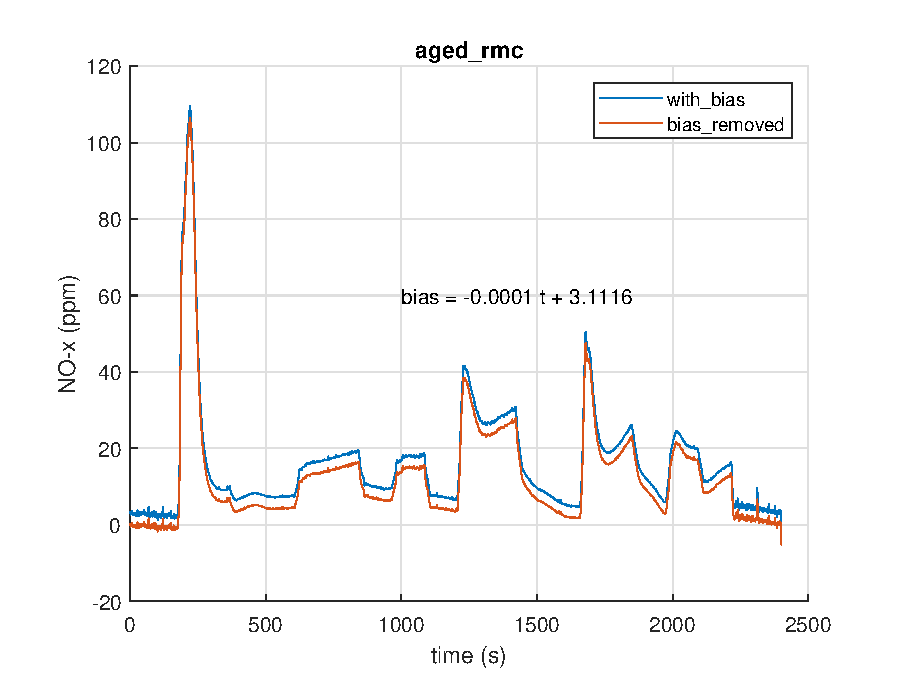
\includegraphics[width=\textwidth]{./figs/chi_est/aged_rmc_NOx_bias.eps}
        \end{figure}
    \end{minipage}
    \begin{minipage}{0.4\textwidth}
        \begin{figure}[H]
            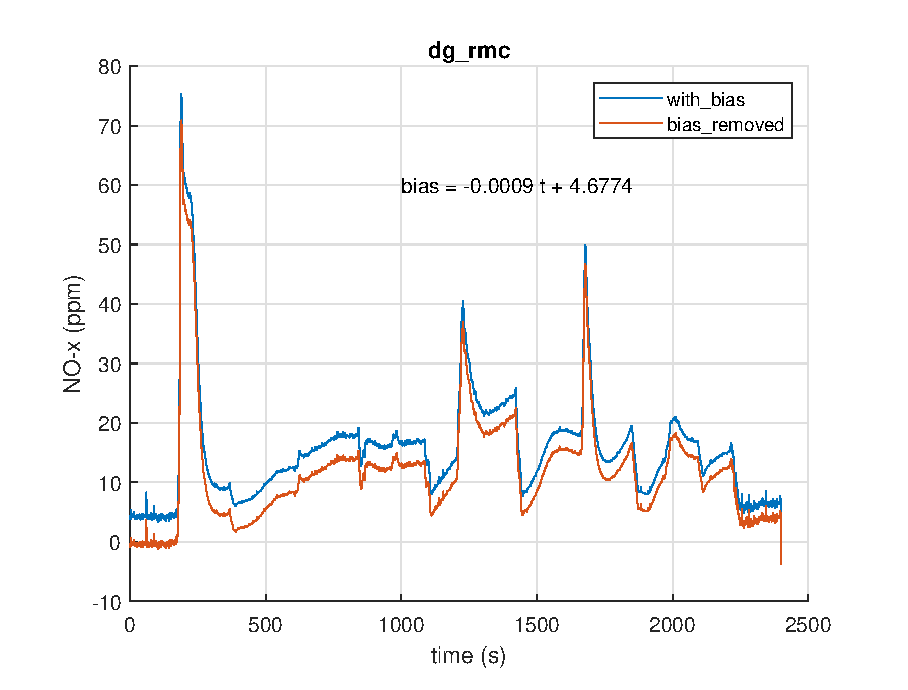
\includegraphics[width=\textwidth]{./figs/chi_est/dg_rmc_NOx_bias.eps}
        \end{figure}
    \end{minipage}
        \caption{Sensor bias correction for RMC cycles}
\end{figure}



\subsubsection{Effect of $NH_3$ sensor bias and minimum threshold for cross-sensitivity}

The ammonia sensor used for ammonia measurement also has bias and there is a
threshold for ammonia sensor for cross-sensitivity to be effective. Thus the
expression for cross-sensitivity becomes:
\begin{align*}
    y_1 &= x_1 + \chi (x_2 - x_{2_{th}})\\
    \implies y_1 &= \bm{x_1 & x_2 & -1} \bm{ 1 \\ \chi \\ \underbrace{\chi \lr{x_{2_{th}}}}_{b}}
\end{align*}

\subsubsection{Least-squares estimation}
\itbf{Assumption}: The temperature changes in RMC cycle don't effect the
cross-sensitivity factor significantly. Thus it can be treated as a constant
w.r.t temperature fluctuations in that range.

We have,
\begin{align*}
    \underbrace{y_1 - x_1}_{\pmb y} &= \underbrace{\bm{x_2 & -1}}_{\pmb \phi^T} \underbrace{\bm{ \chi \\ b}}_{ \pmb \theta}\\
\end{align*}
